\documentclass{article}
\usepackage[utf8]{inputenc}
\usepackage[italian]{babel}
\usepackage[T1]{fontenc}
\usepackage{amsmath}
\usepackage{listings}
\usepackage{color}
\usepackage{graphicx}
\usepackage{enumerate}
\usepackage{adjustbox}
\usepackage{mathtools}
\usepackage{amssymb}
\usepackage{float}
\usepackage{hyperref}
\graphicspath{ {./images/} }

\newcommand{\norm}[1]{\left\lVert#1\right\rVert_2}

\definecolor{dkgreen}{rgb}{0,0.6,0}
\definecolor{gray}{rgb}{0.5,0.5,0.5}
\definecolor{mauve}{rgb}{0.58,0,0.82}

\lstset{emph={getCorrectBit, varOne, varZero, attackerdevice, victimdevice, getrandbits, NUM_TESTS, TimingAttack, EEA, fastExp, testMR, primeGen, __init__, encrypt, decrypt, decryptCRT}, emphstyle=\color{mauve},
        emph={[2]append}, emphstyle={[2]\color{blue}}
        }

\lstset{frame=tb,
  language=Python,
  aboveskip=3mm,
  belowskip=3mm,
  showstringspaces=false,
  columns=flexible,
  basicstyle={\small\ttfamily},
  numbers=none,
  numberstyle=\tiny\color{gray},
  keywordstyle=\color{blue},
  commentstyle=\color{dkgreen},
  stringstyle=\color{mauve},
  breaklines=true,
  breakatwhitespace=true,
  tabsize=3
}


\title{Esercizi Set 2}
\author{Lorenzo Macchiarini}
\date{17 Maggio 2021}

\begin{document}

\maketitle

\section*{Esercizio 2.2: Timing attack contro esponenziazione modulare}
\begin{enumerate}[(a)]
    \item In questo caso dobbiamo studiare la varianza di due Variabili Aleatorie indipendenti     $X$ e $Y$ valori reali di media rispettivamente $\mu_x$ e $\mu_y$:
        \begin{equation}
        \begin{split}
            var(X+Y) &= \mathbb{E}[(X+Y-\mu_x-\mu_y)^2] \\
                     &= \mathbb{E}[(X-\mu_x)^2 + (Y-\mu_y)^2 -2(X-\mu_x)(Y-\mu_y)] \\ 
                     &= \mathbb{E}[(X-\mu_x)^2] + \mathbb{E}[(Y-\mu_y)^2] -2 \mathbb{E}[(X-\mu_x)(Y-\mu_y)]\\
                     &= var(X) + var(Y) - 2cov(X,Y)\\
                     &= var(X) + var(Y)
        \end{split}
        \end{equation}
        Tale risultato si ottiene applicando: al passaggio 3 la linearità del valore atteso, al passaggio 5 il fatto che la covarianza fra due variabili aleatorie indipendenti vale 0.
        
    \item Poiché l'attaccante conosce i bit dell'esponente $d_{k-1}, ... , d_{i+1}$ e ha a         disposizione una copia del dispositivo da attaccare, l'attaccante conosce anche i tempi     di computazione $T'_{k-1}, ... , T'_{i+1}$ uguali a quelli della vittima. L'attaccante     ipotizza il bit $d_i$ della chiave e calcola i tempi di computazione di decryption di      un ciphertext rispetto al dispositivo della vittima, quindi calcola la differenza fra      $T$ e $T'$:
        \begin{equation}
        \begin{split}
            T-T' &= T_{k-1} + ... + T_{i+1} + T_i + ... + T_0 - T'_{k-1} - ... - T'_{i+1} - T'_i \\
                 &= (T_{k-1} - T'_{k-1}) + ... + (T_{i+1}- T'_{i+1}) + (T_i - T'_i) + ... + T_0 \\
                 &= (T_i - T'_i) + ... + T_0 
        \end{split}
        \end{equation}
        L'ultimo passaggio viene ottenuto considerando che i tempi di esecuzione fino al passo $i+1$ sono sicuramente corretti ed uguali a quelli del dispositivo attaccato. Il tempo di computazione $T_i$ richiede un'analisi ulteriore perché potrebbe non essere quello corretto. Se il bit i-esimo fosse corretto, infatti, il risultato sarebbe:
        \begin{equation}
            T-T' = T_{i-1} + ... + T_0 
        \end{equation}
    
    \item Considerando che $var(T_i) = var(T'_i) = v$ possiamo distinguere il calcolo di           $var(T-T')$ in due casi:
        \begin{itemize}
            \item se $d_i = d'_i$ ottengo che $var(T-T') = var(T_{i-1}) + ... + var(T_0) = i \times v$
            \item se $d_i \neq d'_i$ ottengo che $var(T-T') = var(T_i) + var(-T'_i) +var(T_{i-1}) + ... + var(T_0) = (i+2) \times v$ poiché $var(-T'_i)=var(T'_i)=v$
        \end{itemize}
    \item Considerando che sicuramente uno fra $d'_i = 0$ e $d'_i = 1$ è corretto:
        \begin{itemize}
            \item Prendo il $d'$ ottenuto fino al bit i+1 come corretto;
            \item Creo due nuove chiavi, una che pone $d'_i = 0$ e l'altra $d'_i = 1$; 
            \item Calcolo la decryption dello stesso ciphertext con queste due nuove chiavi e con il dispositivo attaccato;
            \item Confronto le due varianze ottenute $var(T-T')$ considerando come $T'$ i tempi di esecuzione delle due nuove chiavi;
            \item Considero corretto il bit i-esimo che rende $var(T-T')$ minore come abbiamo verificato nel punto \textit{c}.
        \end{itemize} 
    \item La legge debole dei grandi numeri afferma che il valore atteso di una variabile          aleatoria converge in probabilità alla media campionaria. Questo vuol dire che se          vengono presi N campioni di una variabile aleatoria (con N abbastanza grande) la media di       questi campioni stima con una certa precisione il valore atteso della stessa variabile     aleatoria. Nel nostro caso quindi possiamo calcolare la varianza $var(T-T')$ scrivendola     come:
        \begin{equation}
            var(T-T') = \dfrac{1}{N}\sum_{i \in [1,N]}{(t^{(i)}-t'^{(i)})^2} - \left(\dfrac{1}{N}\sum_{i \in [1,N]}{t^{(i)}-t'^{(i)}}\right)^2
            \label{eq:variance}
        \end{equation}
        Con $t^{(i)}$ e $t'^{(i)}$ estrazioni delle variabili aleatorie $T$ e $T'$.\\
        Come riportato al punto \textit{d}, le estrazioni di queste due variabili aleatorie consistono nel decifrare particolari ciphertext con i metodi distinti (o con il device attaccato o con quello attaccante). Il numero di ciphertext decifrati deve essere scelto in modo che la precisione della stima sia accurata. Vedremo nell'esercizio 3.3 infatti che tale algoritmo di attacco funziona solamente per numeri relativamente grandi di N (circa 10.000).
    \item L'attaccante, per portare a buon fine l'attacco, dovrà eseguire N decifrature per ogni     differente chiave (o sotto chiave), mentre il dispositivo vittima dovrà eseguire le N       decifrature una sola volta. \\
        L'attaccante inizialmente ha a disposizione una chiave \textit{d} vuota. Partendo dal bit k-1-esimo fino ad arrivare al bit 0, ricava il bit corrente utilizzando l'algoritmo riportato al punto \textit{d}. Quindi esegue la decryption con la chiave trovata e con il dispositivo vittima e confronta i risultati ottenuti per verificare la correttezza della chiave. \label{it:attackTheory}
    \item Nel caso in cui venisse considerato il valore atteso della differenza                     $\mathbb{E}[T-T']$ anziché la varianza, non potremmo più capire se il bit i-esimo           testato sia corretto o meno. Considerando che $\mathbb{E}[T_i] = \mathbb{E}[T'_i] = t$,     distinguiamo i due casi:
        \begin{itemize}
            \item se $d_i = d'_i$ ottengo che $\mathbb{E}[T-T'] = \mathbb{E}[T_{i-1}] + ... + \mathbb{E}[T_0] = (i-1) \times t$
            \item se $d_i \neq d'_i$ ottengo che 
                \begin{equation}
                \begin{split}
                    \mathbb{E}[T-T'] &= \mathbb{E}[T_i] + \mathbb{E}[-T'_i] + \mathbb{E}[T_{i-1}] + ... + \mathbb{E}[T_0] \\
                                     &= \mathbb{E}[T_i] - \mathbb{E}[T'_i] + \mathbb{E}[T_{i-1}] + ... + \mathbb{E}[T_0] \\
                                     &= \mathbb{E}[T_{i-1}] + ... + \mathbb{E}[T_0] \\
                                     &= i \times t
                \end{split}    
                \end{equation}  
                poiché $\mathbb{E}[-T'_i] = - \mathbb{E}[T'_i]$, mentre $var(-T'_i)=var(T'_i)$. Quindi il valore del valore atteso della differenza non ci permette di distinguere se il bit i-esimo è corretto o meno.
        \end{itemize}
\end{enumerate}

\section*{Esercizio 2.4: Common modulus failure}
Dato il modulo \textit{n} comune e i due ciphertext $c_1, c_2$ ottenuti cifrando uno stesso messaggio \textit{m} con le due chiavi pubbliche relative $K_1, K_2$, possiamo svolgere due tipi diversi di attacchi per ottenere il messaggio \textit{m}:
\begin{itemize}
    \item attacco che si basa sul fatto che lo stesso messaggio è stato cifrato utilizzando esponenti pubblici diversi coprimi ma un modulo uguale;
    \item attacco che si basa sul fatto che gli esponenti delle chiavi pubbliche sono molto piccoli (7 ed 11) e che anche i ciphertext ottenuti siano di dimensione $< len(n)$.
\end{itemize}
Nel primo attacco l'idea è quella di utilizzare il teorema di Euclide Esteso in quanto sappiamo che $(e_1, e_2) = 1$. Esistono quindi due numeri $x, y$ tali che $x \times e_1 + y \times e_2 = 1$. L'attaccante può calcolare tali $x,y$ e calcolare, grazie al fatto che sia $c_1$ che $c_2$ sono stati cifrati con lo stesso modulo $n$ e che $m$ è lo stesso in entrambi i ciphertext:  
\begin{equation}
\begin{split}
c_1^x \times c_2^y \mod{n}&= m^{e_1 \times x} \times m^{e_2 \times y} \mod{n}\\
                          &= m^{e_1 \times x + e_2 \times y} \mod{n}\\
                          &= m^1 \mod{n} \\
                          &= m
\end{split}
\end{equation}
Passando quindi ai calcoli da svolgere otteniamo che:
\begin{itemize}
    \item Il teorema di Euclide Esteso ritorna i valori di $x,y$ (prendo $r_0 = e_2, r_1 = e_1$):
        \begin{equation}
        \begin{split}
            r_0 &= q_1 \times r_1 + r_2\\
            11 &= 1 \times 7 + 4\\
            7 &= 1 \times 4 + 3\\
            4 &= 1 \times 3 + 1
        \end{split}
        \end{equation} \nonumber
        \begin{equation}
          \begin{split}
            4 &= 11 - 7\\
            7 &= 1 \times 11 - 7 + 3 \Rightarrow 3 = 2 \times 7 - 11\\
            11 - 7 &= 1 \times 2 \times 7 - 11 + 1 \Rightarrow 1 = 2 \times 11 - 3 \times 7
          \end{split}
        \end{equation} \nonumber
    Quindi $x = -3, y = 2$.
    \item Calcolo:
    \begin{equation}
        \begin{split}
            c_2^y\mod{n} &= pow(c_2,y,n)
        \end{split}
        \end{equation} \nonumber
    Per quanto riguarda $c_1^x\mod{n}$ non è possibile elevare il valore $c_1$ ad una potenza $x < 0$. Considerando $x = -k$ con $k > 0$:
    \begin{equation}
        \begin{split}
            m^{e_1 x+e_2 y} = m^{-e_1 k+e_2 y} &\equiv_n  m^{e_2 y} \times (m^{e_1})^{-k}\\
                                  &\equiv_n  m^{e_2y} \times ((m^{e_1})^{-1})^k\\
                                  &\equiv_n  m^{e_2y} \times (inv(m^{e_1},n))^k\\
                                  &\equiv_n  c_2^y \times (inv(c_1,n))^k\\
                                  &\equiv_n m
        \end{split}
    \end{equation}\nonumber
    Quindi possiamo elevare l'inverso di $c_1$ modulo $n$ (chiamato in questo caso $inv(c_1,n)$ alla potenza $|x|$ chiamata $k$. Moltiplicando quindi $c_2^y \times (inv(c_1,n))^k$ otteniamo $m \mod{n}$ come atteso. Il risultato ottenuto è: $m = 75311$.
    Per calcolare tali valori ho utilizzato uno script Python che utilizza le funzioni \textit{pow} per elevare i valori modulo n e usando la funzione $gmpy2.invert$ per invertire $c_1$ modulo n.
    \begin{lstlisting}
    c1_new = pow(gmpy2.invert(c1, n),3, n)
    c2_new = pow(c2,2,n)
    m = c1_new*c2_new%n # m = 75311
    \end{lstlisting}
\end{itemize}
Nel secondo attacco l'idea è quella di sfruttare la vulnerabilità di RSA \textit{low exponent failure} in cui l'esponente pubblico preso piccolo genera un ciphertext di lunghezza molto minore di n. Nel nostro caso sia $e_1$ che $e_2$ sono piccoli, rendendo quindi fattibile questo attacco. Vediamo infatti come la radice settima e la radice undicesima rispettivamente di $c_1$ e $c_2$, calcolate su \href{https://it.calcprofi.com/calcolatrice-radice-ennesima.html}{\textcolor{blue}{questo}} sito,  risulti uguale a $75311$ come confermato dal primo attacco.

\section*{Esercizio 3.1 Implementazione di algoritmi per crittografia a chiave pubblica}
\begin{enumerate}
    \item \textbf{Algoritmo di Euclide Esteso}: Tale algoritmo permette di calcolare l'MCD fra due numeri interi forniti in ingresso \textit{a} e \textit{b} e i due valori \textit{x} e \textit{y} tali che $MCD = x*a + y*b$. L'algoritmo si basa sull'utilizzo di una variabile \textit{r} contenente i resti di una sequenza di divisioni. In particolare i primi due valori di r sono settati a $r_0 = a$, $r_1 = b$. Fino a quando il resto $r_i \neq 0$ viene svolto il calcolo: $r_{i-2} = q_{i-1} \times r_{i-1} + r_i$. Di particolare interesse per l'implementazione quindi sono le formule:
    \begin{equation}
        r_i = r_{i-2} - q_{i-1} \times r_{i-1}
        \label{eq:r}
    \end{equation}
    \begin{equation}
        q_{i-1} = \left\lfloor \frac{r_{i-2}}{r_{i-1}} \right\rfloor
        \label{eq:q}
    \end{equation}
    Nell'implementazione infatti è stato predisposto un dizionario \textit{r} contenente per ogni indice \textit{i} i valori: 
    \begin{itemize}
        \item in r[i][0] il valore del resto al passo i-esimo;
        \item in r[i][1] e r[i][2] i valori di x e y tali che r[i][0] = r[i][1]*a + r[i][2]*b.
    \end{itemize}
    Il calcolo del resto i-esimo viene svolto come r[i] = r[i-2] - q*r[i-1], in accordo all'Equazione \ref{eq:r} fino a quando r[i][0] != 0. Il calcolo di \textit{q} ad ogni passo invece viene calcolato come q = r[i-2][0]//r[i-1][0] in accordo all'Equazione \ref{eq:q}.
    Al passo finale, in cui r[i][0] == 0, in r[i-1] è presente la tupla [MCD, x, y] che quindi viene ritornata in output. 
    Viene riportato di seguito l'algoritmo implementato in cui come primo ed ultimo passo vengono riordinati a e b in modo che il primo valore sia il maggiore fra i due.
    \begin{lstlisting}
def EEA(a,b):
    r = {}
    if(a > b):
        r[0] = numpy.array([a,1,0])
        r[1] = numpy.array([b,0,1])
    else:
        r[0] = numpy.array([b,1,0])
        r[1] = numpy.array([a,0,1])
    
    i=1
    while r[i][0] != 0:
        i += 1
        q = r[i-2][0]//r[i-1][0]
        r[i] = r[i-2] -q*r[i-1]
    if(a > b):
        return(r[i-1][0],r[i-1][1],r[i-1][2])
    else:
        return(r[i-1][0],r[i-1][2],r[i-1][1])

    \end{lstlisting}
    
    \item \textbf{Algoritmo di Esponenziazione Veloce}: Tale algoritmo velocizza il calcolo di $a^m mod(n)$. L'idea è quella di svolgere $log_2(m)$ moltiplicazioni modulo n anzichè svolgere l'elevamento a potenza e quindi svolgere il modulo. L'algoritmo quindi prevede che l'esponente sia riportato in un array di bit in cui il primo sia il più significativo, nel nostro caso in \textit{mBits}. Quindi scorrendo l'array viene aggiornato il valore \textbf{d} che contiene il valore corretto della potenza al passo corrente; infatti \textit{d} è inizializzato ad 1, ad ogni passo se il bit corrente dell'esponente è 1 d viene elevato alla seconda e moltiplicato per a, altrimenti solamente elevato alla seconda (in entrambi i casi modulo n). Questo garantisce che il valore finale di d sia quello corretto. Nell'algoritmo è stato calcolato anche il valore dell'esponente corretto ma poiché non è necessario per la corretta esecuzione dell'algoritmo, è stato commentato.
    \begin{lstlisting}
def fastExp(a,m,n):
    mBits = [int(k) for k in bin(m)[2:]]
    # c = 0
    d = 1
    for i in mBits:
        d = (d*d)%n
        # c = 2*c
        if(i == 1):
            d = (a*d)%n
            # c += 1
    return d
    \end{lstlisting}
    
    \item \textbf{Test di Miller Rabin}: L'algoritmo sviluppa il test di compositness, ovvero ritorna \textit{True} se il numero intero in ingresso è un numero composto, \textit{False} se il numero è primo. Per fare questo sviluppa due test:
    \begin{itemize}
        \item Se $x^{n-1} \equiv_n 1$ allora \textit{n} è composto per il piccolo teorema di Fermat;
        \item Se $x^2 \equiv_n 1$ ma $x \not\equiv_n -1$ allora \textit{n} è composto per la proprietà dei numeri primi rispetto alle radici quadrate dell'unità.
    \end{itemize}
    L'algoritmo quindi prende in ingresso un numero intero \textit{p} e genera in modo randomico un intero dispari minore di p che chiamiamo \textit{x}. Calcola quindi i numeri \textit{m} ed \textit{r} tali che $n-1 = 2^r \times m$. L'algoritmo quindi svolge r passi in cui viene calcolato il vettore \textit{xVec}: al primo passo calcola un numero $x_0 = x^m mod n$ che verrà aggiunto in xVec[0]; negli r-1 passi successivi al passo i-esimo calcola $x_i = x_{i-1}^2 mod n$ e lo aggiunge in xVec[i]. Per generare il valore di ritorno l'algoritmo valuta il vettore xVec: se $x_0 \neq 1$ e se per nessun $i \in [0,r-1]$ ho $x_i = -1$ allora \textit{p} è un numero composto. Tale algoritmo è dimostrato che circa $\frac{1}{4}$ delle volte potrebbe ritornare un falso negativo, ovvero afferma che un numero è primo anche quando è composto. Per aumentare l'accuratezza dell'algoritmo viene ripetuto il test su un numero \textit{NUM\_TESTS} di x diversi (nel nostro caso 5) in modo da rendere l'errore circa $4^{-NUM\_TESTS}$ (nel nostro caso circa 0,00097).
    \begin{lstlisting}
def testMR(p): 
    NUM_TESTS = 5
    r = ((p-1) & (~((p-1) - 1))) # Calcolo ottimizzato di r
    r = int(math.log2(r))
    m = (p-1)//(2**r)

    composite = False 
    j = 0
    while(j < NUM_TESTS and not composite): 
        x = random.randrange(1, p-1, 2) 
        xVec = [] 
        e = fastExp(x,m,p)
        if(e - p == -1):
            xVec.append(-1)
        else:
            xVec.append(e)
            
        i = 0
        while(i < r):
            e = fastExp(xVec[-1],2,p)
            if(e - p == -1):
                xVec.append(-1)
            else:
                xVec.append(e)
            i += 1
        if(not (xVec[0] == 1 or -1 in xVec[:-1])): 
            composite = True
        j += 1
    return composite
    \end{lstlisting}
    \item \textbf{Algoritmo per la Generazione di Numeri Primi}: L'algoritmo genera un numero intero randomico e verifica che il numero sia primo con il test di Miller Rabin. Se il numero è composto ne genera un altro e lo testa nuovamente fino a quando il numero non è primo.
    \begin{lstlisting}
def primeGen(k):
    p = random.getrandbits(k)
    while(testMR(p)): # testMR ritorna True se p risulta composto
        p = random.getrandbits(k)
    return p
    \end{lstlisting}
    \item \textbf{Schema RSA}: Tale algoritmo di cifratura si basa sull'utilizzo di una chiave pubblica $<N,e>$ ed una chiave privata $\phi_n,d>$ calcolate entrambe con l'utilizzo di due primi \textit{p} e \textit{q}. L'algoritmo infatti viene inizializzato con la funzione \textbf{init} passando come parametro \textit{k} il numero di bit di cui devono essere composti p e q. Viene quindi calcolato $n = p*q$ e $totn = \phi_n = (p-1)(q-1)$. Preso quindi $e = 65537$ si verifica se è coprimo con $\phi_n$, se non lo è \textit{e} viene posto ad un nuovo primo, quindi si calcola d come inverso moltiplicativo di e. L'inverso di e viene calcolato con l'algoritmo di Euclide esteso prendendo il fattore moltiplicativo di e, ovvero l'x tale che $x*e + y*\phi_n = 1$ che modulo $\phi_n$ equivale a d stesso.
    \begin{lstlisting}
def __init__(self, k = 1024):
    self.p = primeGen(k)
    self.q = primeGen(k)
    self.n = self.p*self.q
    self.totn = (self.p-1)*(self.q-1)
    self.e = 65537
    while(EEA(self.e, self.totn)[0] != 1):
        self.e = primeGen(16)
    self.d = EEA(self.e, self.totn)[1]
    if(self.d < 0):
        self.d += self.totn
    \end{lstlisting}
    La funzione \textbf{encrypt} cifra un messaggio m in ingresso. Inizialmente il messaggio viene decodificato da stringa a intero con la funzione \textit{bytes\_to\_long}, viene verificato che l'intero ottenuto sia minore di n e coprimo con n (altrimenti viene aggiunto uno spazio al termine del messaggio), infine viene svolta la codifica utilizzando la funzione di esponenziazione veloce implementata che ritorna $m^e mod n$.
    \begin{lstlisting}
def encrypt(self, m):
    while(bytes_to_long(m.encode()) >= self.n):
        m = m[:-1]
    while(EEA(self.n, bytes_to_long(m.encode()))[0] != 1):
        m += " "
    m = bytes_to_long(m.encode())
    return fastExp(m,self.e,self.n)
    \end{lstlisting}
    Per la fase di decryption sono state implementate due funzioni: una che svolge una decryption standard, l'altra che utilizza il teorema cinese del resto.
    \begin{itemize}
        \item \textbf{decrypt}: Decryption standard del ciphertext c. Presumendo che il ciphertext in ingresso sia un numero intero viene svolta la decodifica utilizzando la funzione di esponenziazione veloce implementata che ritorna $c^d mod(n)$:
        \begin{lstlisting}
def decrypt(self, c):
    return fastExp(c,self.d,self.n)
        \end{lstlisting}
        \item \textbf{decryptCRT}: Funzione di decryption che utilizza il Teorema Cinese del Resto. L'utilizzo di questo metodo permette di velocizzare molto la fase di decryption in quanto non viene calcolato $c^d mod(n)$ ma una versione con moduli molto minori (con p e q). Per questo teorema quindi posso calcolare il risultato di $c^d mod(n)$ come soluzione del sistema
        \begin{equation}
        \begin{cases}
            X &\equiv_p c^d \\
            X &\equiv_q c^d
        \end{cases}
        \end{equation}
        Poiché sia p che q sono primi posso ridurre l'esponente modulo p-1 o q-1 e ridurre anche c modulo p o q.
        \begin{equation}
        \begin{cases}
            X &\equiv_p (c\%p)^{d\%(p-1)}\\
            X &\equiv_q (c\%q)^{d\%(q-1)}
        \end{cases}
        \end{equation}
        La soluzione del sistema è quindi ottenuta calcolando i valori da moltiplicare ad ognuno dei due termini:
        \begin{equation}
            c_p = \frac{p*q}{p} \times \left[\left(\frac{p*q}{p}\right)^{-1} \% p\right] = q \times [q^{-1} \% p]
        \end{equation}
        \begin{equation}
            c_q = p \times [p^{-1} \% q]
        \end{equation}
        In cui le potenze negative rappresentano gli inversi modulo il modulo che le segue. Questi due valori \textit{cp, cq} sono calcolati nella funzione di inzializzazione di RSA come:
            \begin{figure}[t]
    \centering
    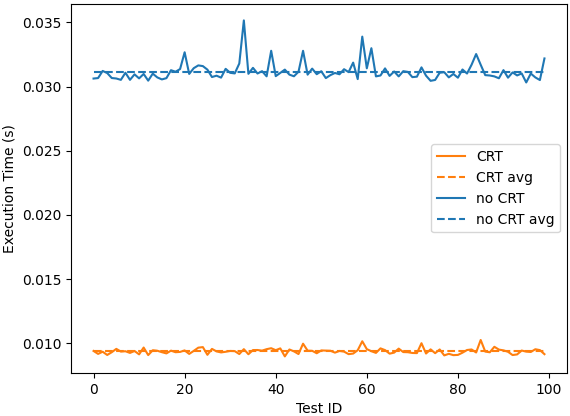
\includegraphics[width=10.1cm]{images/CRT.png}
    \caption{Grafico che mostra l'esecuzione di 100 decifrature RSA di ciphertexts diversi con il Teorema Cinese del Resto (in arancione) e senza (in blu). Viene anche riportato il valore medio delle due esecuzioni: 0,009 con CRT e 0,03 senza CRT.}
    \label{fig:CRT}
    \end{figure}
        \begin{lstlisting}
self.cp = self.q*(EEA(self.q,self.p)[1] % self.p)
self.cq = self.p*(EEA(self.p,self.q)[1] % self.q)
        \end{lstlisting}
        La funzione di decryption quindi risulta per quanto scritto:
        \begin{lstlisting}
def decryptCRT(self, c):
    dp = fastExp(c%self.p,self.d%(self.p-1),self.p) 
    dq = fastExp(c%self.q,self.d%(self.q-1),self.q) 
    return (dp*self.cp + dq*self.cq )% self.n 
        \end{lstlisting}
    \end{itemize}
    Ho confrontato i tempi di esecuzione dei due algoritmi di decryption nella Figura \ref{fig:CRT} in cui sono riportati i tempi di 100 esecuzioni delle due implementazioni con ciphertext diversi. Vediamo che il valor medio dei tempi di esecuzione della decryption con il CRT è circa $0,009s$ mentre senza il CRT è circa $0,03$ ovvero circa 3 volte. Per generare ciphertexts diversi ho generato 100 plaintexts casuali di lunghezza $2^8$ caratteri e li ho cifrati ottenendo quindi i 100 ciphertexts da fornire in input ai due algoritmi.

\end{enumerate}

\section*{Esercizio 3.3 Timing attack}
L'obiettivo di tale esercizio è mostrare che lo studio svolto nell'Esercizio 2.2 sia corretto. In particolare in questo caso :
\begin{itemize}
    \item il dispositivo vittima è rappresentato dalla funzione \textit{ta.victimdevice(c)} che prende in input il ciphertext da decifrare e ritorna il tempo di computazione;
    \item il dispositivo attaccante è rappresentato dalla funzione \textit{ta.attackerdevice(c,v)} che prende in input il ciphertext da decifrare e la chiave (o sotto chiave) da utilizzare per la decifratura e ritorna il tempo di computazione;
\end{itemize}
In entrambi questi "dispositivi" viene utilizzato il metodo di esponenziazione veloce per la decryption che permette l'esecuzione del Timing Attack. %TODO scrivere dell'alg di exp veloce? Dipendente da se bit = 1 fa 2 op, altrimenti 1
Seguendo le direttive scritte nel Punto \ref{it:attackTheory} dell'Esercizio 2.2, i passi dell'algoritmo sono:
\begin{itemize}
    \item Genero casualmente un insieme di ciphertexts di dimensione \textit{NUM\_TESTS} che saranno gli input da dare alle funzioni per ottenere N campioni di ogni variabile aleatoria tempo di esecuzione (del dispositivo vittima e delle varie iterazioni del dispositivo attaccante con diverse chiavi private $d'$);
    
    \begin{lstlisting}
ciphertexts = []
for i in range(NUM_TESTS):
    ciphertexts.append(random.getrandbits(100))
    \end{lstlisting}
    
    \item Calcolo quindi gli N tempi di esecuzione del dispositivo vittima relativi alle decryption degli N ciphertexts e li mantengo costanti per tutta l'esecuzione dell'attacco;
    
    \begin{lstlisting}
ta = TimingAttack()
correctTimes = []
for i in range(len(ciphertexts)):
    correctTimes.append(ta.victimdevice(ciphertexts[i]))
    \end{lstlisting}
    
    \item Partendo dalla chiave $dFound = [1]$ calcolo i 63 bit rimanenti della chiave uno ad uno partendo dal bit più significativo. In particolare ad ogni iterazione:
    \begin{itemize}
        \item Genero due vettori \textit{dZero} e \textit{dOne} contenenti i bit di \textit{dFound} e con il bit relativo all'iterazione corrente $dZero[i] = 0$ e $dOne[i] = 1$;
        \item Calcolo gli N tempi di esecuzione relativi ai due vettori ottenuti;
        \begin{lstlisting}
zeroTime = []
oneTime = []
for j in range(len(ciphertexts)):
    zeroTime.append(ta.attackerdevice(ciphertexts[j],dZero))
    oneTime.append(ta.attackerdevice(ciphertexts[j],dOne))
        \end{lstlisting}
        \item Confronto i risultati dei tempi ottenuti con la funzione \textit{getCorretBit} che prende in ingresso il vettore dei tempi della vittima e i vettori dei tempi delle due versioni e ritorna in output il valore del bit corretto calcolato.
        \begin{lstlisting}
dFound.append(getCorrectBit(correctTimes,zeroTime,oneTime))
        \end{lstlisting}
    \end{itemize}
    \item Per verificare che la chiave \textit{dFound} sia corretta utilizzo la funzione \textit{ta.test()} che mostra se la chiave trovata ha un numero di bit uguali a quelli della chiave della vittima $< 75\%$, compreso fra $75\%$ e $100\%$ o proprio il $100\%$. In un contesto reale è possibile svolgere un test analogo confrontando il risultato della decifratura con la chiave trovata rispetto alla decifratura della vittima; se il risultato è uguale allora la chiave ha il $100\%$ di bit corretti. 
\end{itemize}
Di particolare interesse è la funzione \textit{getCorretBit(correct, zero, one)} in cui come input vengono forniti i tempi di esecuzione della vittima (correct) e delle due versioni testate in cui i primi i-1 bit più significativi sono corretti mentre il bit i-esimo assume i valori 0 (zero) e 1 (one) al variare delle due versioni. Il test si basa sul calcolare le varianze del valore T-T', ovvero la differenza fra i tempi dell'algoritmo che usa l'esponente corretto e quelli dell'algoritmo che usa le due versioni dell'esponente. In output quindi viene restituito il bit i-esimo corretto in base a quale delle due versioni genera il valore di varianza minore. In questa implementazione ho calcolato la varianza utilizzando la Formula \ref{eq:variance} ed in particolare calcolando le due sommatorie in modo separato (la prima nella posizione [0] e la seconda nella posizione [1] dei vettori \textit{varianceZero} e \textit{varianceOne}). Al termine del calcolo delle due varianze confronto i valori e scelgo quello minore in accordo a quanto riportato al punto \ref{it:attackTheory} dell'Esercizio 2.2.
\begin{lstlisting}
def getCorrectBit(correct, zero, one):
    varianceZero = [0,0] 
    varianceOne = [0,0]
    
    for i in range(len(correct)):
        varianceZero[0] += (correct[i] - zero[i])**2
        varianceZero[1] += correct[i] - zero[i]
        varianceOne[0] += (correct[i] - one[i])**2
        varianceOne[1] += correct[i] - one[i]
        
    varianceZero[0] /= len(correct)
    varianceZero[1] /= len(correct)
    varianceZero[1] = varianceZero[1]**2
    varZero = varianceZero[0] - varianceZero[1]
    
    varianceOne[0] /= len(correct)
    varianceOne[1] /= len(correct)
    varianceOne[1] = varianceOne[1]**2
    varOne = varianceOne[0] - varianceOne[1]
    
    if(varZero < varOne):
        return 0
    return 1
\end{lstlisting}
Ho notato che la correttezza della chiave trovata è strettamente dipendente dal numero di campioni di ciphertext forniti. In particolare possiamo vedere in Tabella \ref{tab:correctness} che per valori di $NUM\_TESTS <1000$ quasi sicuramente la stima della varianza non è corretta, per $1000 < NUM\_TESTS < 2600$ la stima inizia ad assestarsi ma può avere ancora errori, $2600 < NUM\_TESTS$ la stima ha una precisione sufficiente da permettere la buona riuscita dell'attacco.

\begin{table*}[t]
    \hskip-4.45cm
        \begin{tabular}{ c || c | c | c | c | c | c | c | c | c | c | c | c | c | c | c }
         Test&200&400&600&800&1000&1200&1400&1600&1800&2000&2200&2400&2600&2800&3000\\\hline \hline
         I&$<\!75\%$&$<\! 75\%$&$< \!75\%$&$< \!75\%$&$100\%$&$100\%$&$<\! 75\%$&$100\%$&$100\%$&$100\%$&$100\%$&$100\%$&$100\%$&$100\%$&$100\%$\\ \hline
         
         II&$<\! 75\%$&$< \!75\%$&$<\! 75\%$&$< \!75\%$&$< \!75\%$&$< \!75\%$&$100\%$&$100\%$&$100\%$&$100\%$&$100\%$&$<\! 75\%$&$100\%$&$100\%$&$100\%$\\  \hline
         
         III&$< \!75\%$&$<\! 75\%$&$<\! 75\%$&$<\! 75\%$&$< \!75\%$&$100\%$&$100\%$&$100\%$&$100\%$&$100\%$&$100\%$&$100\%$&$100\%$&$100\%$&$100\%$\\ \hline
         
         IV&$< \!75\%$&$<\! 75\%$&$< \!75\%$&$< \!75\%$&$<\! 75\%$&$100\%$&$100\%$&$100\%$&$100\%$&$100\%$&$100\%$&$100\%$&$100\%$&$100\%$&$100\%$\\\hline 
         V&$< \!75\%$&$< \!75\%$&$< \!\!75\%$&$<\! 75\%$&$< \!75\%$&$< \!75\%$&$100\%$&$100\%$&$100\%$&$<\! 75\%$&$100\%$&$100\%$&$100\%$&$100\%$&$100\%$\\
         
        \end{tabular}
    \caption{Tabella che mostra come all'aumentare del numero di campioni di ciphertext con cui calcolare la stima della varianza, aumenta la probabilità che il Timing Attack dia esito positivo. In particolare vengono riportati i casi in cui la chiave trovata abbia un numero di bit corretti $< 75\%$ o $ = 100\%$. Notiamo come con circa 3000 campioni è quasi sicuro che la chiave sia corretta.}
    \label{tab:correctness}
\end{table*}

\end{document}
